\documentclass[12pt]{article}

\usepackage{sbc-template}
\usepackage{graphicx,url}
\usepackage[utf8]{inputenc}
\usepackage[brazil]{babel}
\usepackage{float}
%\usepackage[latin1]{inputenc}  

     
\sloppy

%% \title{Instructions for Authors of SBC Conferences\\ Papers and Abstracts}
%%\title{Modelo de Apoio ao Ensino em Ambientes Virtuais de Aprendizagem Sustentado por Consciência Situacional}
\title{Consciência Situacional em Ambientes Virtuais de Aprendizagem:
	Modelo Mental Proposto em Obras de Mineração de Dados Educacionais }

\author{Ernani Martins\inst{1}, Luciana Assis\inst{2}, Cláudia Berti\inst{2}, Alessandro Vivas\inst{2} }


\address{Instituto de Informática -- Universidade Federal do Rio Grande do Sul
  (UFRGS)\\
  Caixa Postal 15.064 -- 91.501-970 -- Porto Alegre -- RS -- Brazil
\nextinstitute
  Departamento de Computação \\ Universidade Federal dos Vales do Jequitinhonha e Mucuri (UFVJM) \\
  Diamantina, MG -- Brazil
  \email{\{naninmartins,lupassis,claudiabberti,alessandro.vivas\}@gmail.com}
}

\begin{document} 

\maketitle

\begin{abstract}
  This article describes the use of Situational Awareness (CS) in support of Virtual Learning Environments (AVA's). Educational Data Mining (EDM) researches the development of methods for data processing generated from educational environments, however AVA's tend to result in extremely dynamic datasets, thus requiring tools that adapt to the variations arising from each interaction with the user. The CS uses Mental Models to systematically assimilate states in certain situations, the conscious view about the environment allows the identification of each configuration of the data and what better action to take, being able to delimit situations in which the MDE methods best apply.
\end{abstract}
     
\begin{resumo} 
  Este artigo descreve o uso da Consciência Situacional (CS) no suporte à Ambientes Virtuais de Aprendizagem (AVA's). Mineração de Dados Educacionais (MDE) buscam o desenvolvimento de métodos para processamento de dados gerados a partir de ambientes educacionais, no entanto AVA's tendem a resultar em conjuntos de dados extremamente dinâmicos, requerendo assim ferramentas que se adaptem as variações decorrentes de cada interação com o usuário. A CS usa Modelos Mentais para assimilar sistematicamente estados em determinadas situações, a visão consciente sobre o ambiente permite a identificação de cada configuração dos dados e qual melhor ação a ser tomada podendo delimitar situações nos quais os métodos da MDE melhor se aplicam.
\end{resumo}


\section{Introdução} 

O recente aprimoramento da tecnologia tem fornecido grande flexibilidade aos educadores para disseminar o conhecimento nas mais inúmeras plataformas. \cite{Ahmad_Shamsuddin_2010} afirmam que o uso destas tecnologias disponibilizam diversas abordagens para facilitar o ensino, maximizando os resultados de aprendizagem entre os discentes.

Ambientes Virtuais de Aprendizagem (AVA's) criam modelagens e diretrizes que possam inferir o estado do aprendizado de cada estudante, assim modalidades de ensino da Educação a Distância caracterizam-se por práticas pedagógicas personalizadas utilizando-se das mais diversas tecnologias da informação em vários graus educacionais. 

A utilização das plataformas pelos discentes resulta em um conjunto diverso de dados em inúmeras situações de interação com o ambiente, este valor numeroso de dados pode dificultar o gerenciamento e análise sobre a relação dos agentes junto dos AVA's \cite{Rabelo_et_al2017}. Alunos e professores relacionam-se por meio da disponibilização de materiais, discussão em fóruns sobre determinados assuntos e chats, todavia, estes meios por vezes não são o bastante para que os discentes consigam atingir o conhecimento em sua melhor forma \cite{Falci_et_al_2018}. 

\cite{Endsley2012} enfatizam que o grande volume de dados em sua maioria não permitem extrair um conhecimento sucinto e real da situação. A dinamicidade dos acontecimentos no ambiente deverá ser capturada e assimilada em um processo ininterrupto, integrando a percepção dos elementos no espaço, assim como a compreensão e projeção de eventos imediatamente no futuro \cite{Silva_et_al_2012}.

O entendimento de aspectos existentes no ambiente é chamado de Consciência Situacional-CS (do inglês Situation Awareness), \cite[p.13]{Endsley2012} compreendem a CS em `` estar ciente do que está acontecendo ao seu redor e entendendo o que estas informações significam agora e no futuro ". 

\cite{Roy_Breton_Rousseau_2007} afirmam que a CS é um componente natural da organização cognitiva humana, e os benefícios que resultam de um melhor entendimento da situação podem ser percebidos desde a pré-história. Uma Decisão assertiva torna-se difícil quando não existe uma boa consciência da situação \cite{Endsley2012}. 

Técnicas e tecnologias baseadas em Mineração de Dados Educacionais (MDE) e a CS podem facilitar o processo de Tomada de Decisão e entendimento do ambiente, possibilitando assim a construção de sistemas com conteúdo adaptativo ao processo de aprendizagem do aluno. A MDE emprega diversas técnicas e procedimentos sobre uma base de dados educacional desejando a descoberta de conhecimento relevante. 

\cite{Endsley1995} e \cite{Endsley2012}  relatam que a CS emprega Modelos Mentais na criação de estruturas complexas  para mapear o comportamento de sistemas específicos diminuindo assim a carga de dados sobre um usuário. Este arcabouço de situações sugere qual procedimento a ser tomado dada determinada situação. 

Modelos Mentais podem auxiliar na escolha dos métodos de MDE sobre determinadas circunstâncias, o resultado do processamento destes métodos influencia diretamente no nível de CS que o ambiente educacional atingirá. 

\section{Fundamentação Teórica} \label{sec:firstpage}
	
Este capítulo provê uma base teórica referente a formalização dos conceitos de Consciência Situacional e Mineração de Dados voltado a educação, em razão de facilitar o processo de tomada de decisão em ambientes educacionais.  

\subsection{Consciência Situacional}

\cite [p. 97]{Endsley1988} define CS como: `` a percepção dos elementos no ambiente dentro de um volume de tempo e espaço, a compreensão dos seus significados, e a projeção dos seus estados em um futuro próximo ".

A falta de CS leva as pessoas a um desentendimento da situação em que se encontram, sendo que a melhor maneira de auxiliar a avaliação humana é suprindo o usuário com altos níveis de Consciência Situacional \cite{Endsley2012}. Todas as tarefas cotidianas requerem níveis específicos de consciência, ao cozinhar por exemplo, a pessoa deve entender todos os parâmetros do ambiente, como temperatura da panela, quantidade de água esquentando, previsão de fervura da água e etc.

Existem algumas variações nos modelos de definição da consciência da situação, contudo a definição melhor aceita na literatura para modelagem computacional foi proposta por \cite{Endsley1995} sendo separados em 3 níveis: \emph{percepção, compreensão e projeção}.

\begin{itemize}
		
	\item \textbf{\textit{Percepção} dos elementos do ambiente:}
	
	Neste estado é necessário perceber os sinais do ambiente, variáveis relevantes, elementos e atributos do ambiente, é o primeiro passo para obtenção da Consciência Situacional. Sem uma boa percepção, informações relevantes as etapas de compreensão e projeção ficam incompletas, levando a interpretações ruidosas e baixa consciência sobre os estados do ambiente.
	
	\item  \textbf{\textit{Compreensão} da situação atual:}
	
	O segundo passo na obtenção da CS é conseguir realizar o entendimento mais correto possível sobre os dados colhidos, compreendendo as relações e dinamismos percebidas em sinais que serão relevantes para alcançar os objetivos. Baseado em conhecimentos dos elementos do nível 1, o tomador de decisão reconhece padrões e formas em uma figura holística do ambiente, compreendendo a significância dos objetos e eventos.	
	
	\item \textbf{\textit{Projeção} do estado futuro:}
	
	Nesta etapa deve-se ser capaz de predizer um estado futuro, ou seja, a habilidade de antever eventos onde tomadores de decisão necessitam de um alto nível de SA. O Nível 3 somente é obtido a partir de uma boa compreensão (Nível 2), assim os dados compreendidos fornecem a ciência necessária para antecipar fatos que possam vir a ocorrer.
	
\end{itemize}

\subsection{Modelos Mentais}

Para \cite{Endsley2012} o indivíduo  possui dois tipos de memórias: \textit{de curto prazo ou de trabalho e de longo prazo}. Quando armazenamos informações em \textit{memória de trabalho}, gravamos o conhecimento em uma base temporária na mente, entretanto somente uma quantia restrita de informação consegue ser retida e manipulada, sendo que uma pessoa deverá relacionar-se ativamente com estas informações para não esquecê-las. A informação conciliada com conhecimento prévio em uma memória de trabalho cria uma nova imagem mental ou a atualiza conforme mudanças na situação. 	

Imagens mentais são formas de representar em pensamento o mundo externo, a mente humana capta o mundo exterior a partir de representações mentais. Estas visões podem ser categorizadas entre representações \textit{analógicas e proposicionais}, a imagem visual é um exemplo de representação analógica \cite{Moreira1996}. 

Por outro lado as representações proposicionais são abstratas, organizadas em regras rígidas compreendendo o conteúdo ideacional da mente. Estas representações proposicionais mapeiam-se em uma linguagem da mente (`` mentalês "), de forma que representações proposicionais não são pensamentos expressos em frases, mas sim entidades individuais e abstratas formuladas em linguagem própria da mente, alguns psicólogos cognitivos afirmam que a imagem mental pode ser reduzida a representações proposicionais  \cite{Moreira1996}.

Memórias de longo-prazo estruturadas podem ser utilizadas para contornar as limitações em memórias de trabalho, gerenciando o conhecimento em modelos mentais, esquemas e scripts, desempenhando uma importante função na CS \cite{Endsley1995}. 

 Modelos Mentais foram definidos por \cite[p.60]{Rouse1985} apud \cite{Endsley1995} como: `` mecanismos pelos quais humanos são capazes de gerar descrições e formas de sistemas propostos, explicações de funcionalidades e estados observados do sistema, e previsões de estados futuros ".

Um \textit{esquema} é um estado provável em que podemos acessar a partir de um modelo mental, a mente define padrões de acontecimentos anteriores e os reconhecessem conforme as entradas do ambiente \cite{Endsley2012}. 

Os esquemas podem funcionar como atalhos para que não necessitemos acessar o modelo mental a todo momento, (como se tivéssemos uma sensação de \textit{dejavú}). Estes esquemas são formados a partir de casos vividos, contudo, uma vantagem dos esquemas são que não necessitam representar exatamente outras situações parecidas pois as pessoas tem a capacidade de relacionar características de uma situação com um esquema \cite{Endsley2012}.

Um \textit{script} são sequências de ações sendo associadas a um esquema,ou seja, são passos do que se deve fazer a partir da seleção de uma ação, os scripts também são desenvolvidos a partir da experiência, ou são normatizados pelo domínio. Um doutor ao selecionar um esquema (determinando um estado do paciente), trabalhará com passos bem definidos executando uma série de ações pré-programadas dada a resposta clínica do paciente à cada procedimento \cite{Endsley2012}.  

\cite{Moreira1996} acredita que não existe um único modelo mental para determinadas situações ou estados em uma mesma abordagem dos fatos, ainda que um modelo mental demonstre-se mais adequado para representação da situação. Um mecânico pode seguir trocando entre vários modelos mentais e esquemas conforme segue na identificação das entradas (possíveis problemas) do seu exame no carro.

\subsection{Mineração de Dados Educacionais}

A Mineração de Dados foi desenvolvida com o intuito de permitir descoberta de conhecimento sobre uma base de dados. \cite{Goldschmidt_Passos_2005} afirmam que este conjunto de técnicas oriundas da Estatística e Inteligência Artificial visam obter conhecimento novo, útil, relevante e não-trivial os quais possam estar escondidos em tais bases.

\cite{Leite_et_al_2016} reforçam que o uso de técnicas de Mineração de dados ao contexto educacional ou MDE (Mineração de Dados Educacionais) são soluções promissoras para a compreensão de informações nas base de dados em AVA's.

\cite{Romero_Ventura_2013} concordam em dizer que MDE pode ser definida como a aplicação de técnicas de MD para o específico tipo de conjunto de dados originados em ambientes educacionais, combinando ciência da computação, estatística e educação .

\cite{Garcia_et_al_2011} e \cite{Santos2016} elucidam o processo de MDE em uma conversão de dados brutos de Sistemas Educacionais em informação, que podem ser usadas por desenvolvedores de software, professores, pesquisadores educacionais, em informação útil. \cite{Garcia_et_al_2011} ressaltam que o processo de mineração de dados educacionais é baseado nos mesmos passos de um processo de MD.

\section{Estado da Arte}

\cite{Dorca2012} desenvolve uma abordagem estocástica visando a detecção dos Estilos de Aprendizagem do aluno, o desenvolvimento do trabalho resultou em um Módulo do Estudante, um Módulo Pedagógico e o Componente de Modelagem do Estudante. O autor aplica a Cadeia de Markov e Algoritmo de Aprendizagem por Reforço como técnicas dentro dos módulos para o processo de detecção do estilo.

\cite{Salazar_Vivas_Luciana_2017} construíram um novo algoritmo empregando o uso de redes Bayesianas para detecção do estilo de aprendizagem, \cite{Falci_et_al_2018} propõem uma customização desta abordagem utilizando lógica fuzzy e categorização de reforços, já \cite{Ribeiro_et_al_2017} aplicam o uso de Média Móvel Exponencialmente Ponderada para detecção dos estilos.

\cite{Sena_etal_2016} usam cadeias ocultas de Markov com o algoritmo Virtebi procurando potencializar o processo de seleção dos Estilos de Aprendizagem dos alunos, \cite{Silva_etal_2017} utilizam a técnica de Aprendizagem de Máquina online \texttt{Dynamic Scripting} no lugar do algoritmo de Aprendizagem por Reforço usado por \cite{Dorca2012}.

\cite{Falci_et_al_2016} propõem um algoritmo novo para que o sistema convirja para o estilo de aprendizagem mais rápido do que a técnica de Aprendizagem por Reforço a partir de uma análise dos históricos da Categorização do Estilo de Aprendizagem .

\cite{Ahmad_Shamsuddin_2010} fazem uma análise comparativa das Técnicas de Mineração para Detecção Automática dos Estilos de Aprendizagem do Estudante, os autores utilizam nove algoritmos diferentes baseados em três técnicas de mineração: regras de associação, redes Bayesianas e árvores de decisão, presentes dentro da ferramenta Weka, concluíram por fim que algoritmos baseados em árvores de decisão apresentaram substancial porcentagem de acurácia comparados a redes Bayesianas e regras de associação.

\cite{Fernandes2017} utilizou-se do Algoritmo de  Classificação Associativa em MDE na previsão do desempenho de estudantes no combate a evasão da EAD. O estudo dividiu-se em 4 experimentos: algoritmo CBA usando o algoritmo Apriori, algoritmo CBA com Predictive Apriori, Balanceamento das Classes de estudo antes da aplicação dos algoritmos e Cortes Temporais, objetivando a divisão do conjunto de dados em períodos temporais de forma que os professores obtivessem resultados progressivos dos estudantes.

\cite{Dias_e_Filho_etal_2008} a partir da avaliação dos dados do ambiente LabSQL desenvolveram tarefas de classificação aplicando Redes Bayesianas e Árvores de decisão, buscando entre os dados relacionamentos novos não previstos. As árvores de decisão deixaram a mostra padrões referentes ao processo de aprendizado relacionado ao comportamento dos alunos. 

\cite{Mitsch_et_al_2013} realizaram uma pesquisa de técnicas de MD concentrada em clusterização para o uso em Consciência Situacional, o autor ressalta a especificidade dos requisitos necessários para a CS, dada a natureza destes sistemas em lidar com uma faixa larga de heterogeneidade em objetos inter-relacionados oriundos de várias fontes, propondo assim um critério de avaliação entre CS e MD para seleção de técnicas de clusterização espaço-temporais.

\cite{Yin_et_al_2012} modelaram o uso da Consciência Situacional para avaliar Situações de Emergência atráves de sensores oriundos de Mídias Sociais, usando processamento de linguagem natural e técnicas de MD para extrair informações no Twitter geradas a partir de desastres e crises.

\cite{Krishnaswamy_et_al_2005} desenvolvem uma arquitetura que busca a CS em rodovias, para isto, propõe-se o uso de técnicas de mineração de dados onipresentes embarcadas em dispositivos móveis transmitidas em redes wireless dispostas nas rodovias. A arquitetura promete reduzir erros humanos graças ao monitoramento das estradas e dos dispositivos móveis dentro dos carros executando o algoritmo LWC de classificação de eventos.

\section{Abordagem Proposta}

O presente trabalho propõe uma organização computacional de um Modelo Mental que poderá ser aplicado diretamente sobre as etapas de Compreensão e Projeção na construção de AVA's suportados por CS, tais softwares devem ter a capacidade de auto-gerenciamento definindo assim qual melhor técnica de MDE deverá ser tomada diante de cada situação.

A estrutura do Modelo Mental deverá ser capaz de avaliar as características dos dados a serem processados, objetivo a ser atingido e a condição encontrada no estado vigente. Os esquemas e scripts deste modelo desempenham papel crucial relacionando todas as características da situação presente a alguma estrutura vivenciada e/ou definida anteriormente.

Em uma situação empírica ótima os modelos mentais deveriam ser capazes de sugerir quais possíveis melhores métodos incorporados a MDE adequam-se para obtenção do resultado esperado. 

O Modelo Mental é volátil e pode ser alterado futuramente conforme a mudança das condições do ambiente onde o software funcionará, os objetivos são extremamente dinâmicos e ilustram as metas do ambiente no qual foram inseridos. O Modelo aqui proposto fundamenta-se nos objetivos, características do conjunto de dados e métodos nos estudos realizados pelas obras levantadas neste trabalho. Os objetivos são: Detecção do Estilo de Aprendizagem e Prevenção do Desempenho acadêmico do Discente.

A organização a ser seguida pelo Modelo Mental poderá ser construída em diversas estruturas computacionais de dados, decidiu-se neste trabalho o uso de Árvores de Decisão devido a sua facilidade de entendimento e implementação (Figura \ref{arvoreDecisao}). 

O parâmetro de entrada na árvore indica qual o objetivo da iteração será explorado no conjunto de dados, desta definição, percorre-se o caminho que melhor atende as expectativas e características do conjunto, deduzindo através de experiências prévias qual técnica em MDE possivelmente melhor se encaixa ao conjunto (ex: Em Detecção do Estilo de Aprendizagem, se o tratamento dos dados é Estocástico e o nº de iterações é pequeno então deverá ser aplicado o algoritmo de Virtebi como expõem \cite{Sena_etal_2016}). 


\begin{figure}[H]
	\centering
	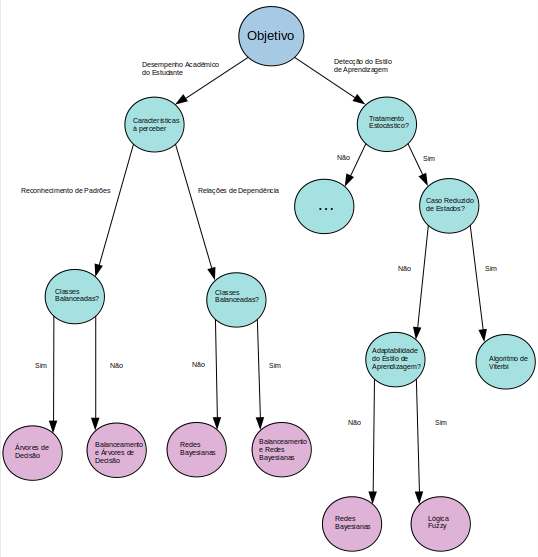
\includegraphics[scale=0.85]{figuras/ArvoreDecisao}
	\caption{Árvore de Decisão para seleção de metódo MDE. Fonte: elaborado pelo autor }
	\label{arvoreDecisao}	
\end{figure}

\section{Discussões}

O Modelo Mental procura representar o máximo de eventos que melhor atendam as situações comuns sobre um conjunto de dados. Para cada tarefa a ser executada em um AVA deve existir situações previamente estruturadas que se assemelham aos padrões da iteração, do contrário esta nova situação deverá ser avaliada e possivelmente adicionada ao modelo.

Aplicando diretamente sobre as etapas de Compreensão e Projeção em CS os modelos exercem diferentes papéis em cada etapa. Em Compreensão os modelos mentais atuam comparando a iteração corrente com esquemas e scripts que melhor aplicam-se naquele conjunto de dados a partir do objetivo selecionado pelo docente.

\begin{itemize}	
	\item \textit{Para a situação ``\textbf{Y}" geralmente o método ``\textbf{X}" tem apresentado melhores resultados!}
\end{itemize}

Por sua vez os modelos mentais atuam na etapa de Projeção descrevendo o cenário, evidenciando os estados observáveis e atingíveis fundamentados pelos conhecimentos evidenciados no estágio anterior, ou seja, antevem cenários atingidos pelos alunos diante das relações criadas entre os dados do sistema.

\begin{itemize}	
	\item \textit{Se existe o relacionamento ``\textbf{Z}" e a variável ``\textbf{Y}" é maior do que ``\textbf{X}", geralmente atinjo o estado ``\textbf{K}"!}
\end{itemize}

Um modelo mental pode influenciar as etapas de Compreensão e Projeção simultaneamente, ou agir especificamente em cada etapa do processo. O modelo aqui representado (figura \ref{arvoreDecisao}) atua diretamente sobre a etapa de Compreensão em CS.


\section{Considerações Finais}

O uso da CS viabiliza um entendimento mais sucinto e claro das ações em execução no ambiente, assim no âmbito educacional o seu uso traz uma perspectiva mais ampla sobre as inúmeras respostas coletadas naquela esfera. Este processo viabiliza a maior assertividade nas ações tomadas por discentes uma vez que estes estejam mais conscientes sobre o estado deparado no ambiente.

Este trabalho desenvolve um modelo mental estruturado em Árvore de Decisão para que possa ser implementado em AVA's, tal modelo estrutura-se nas experiências e características relatas pelos trabalhos aqui referenciados. 

Atuando diretamente sobre a etapa de Compreensão dos dados, a árvore procura otimizar a extração de conhecimento do conjunto de dados educacionais. O modelo mental procura expandir o uso das técnicas da mineração de dados, pois propõe à aplicação o método que melhor se adapta ao estado do ambiente.

Esta pesquisa limitou-se a utilização de técnicas MDE para o processamento dos dados, entretanto pode-se expandir a outras abordagens para a descoberta do conhecimento, o uso de linguagens lógicas e ontologias por exemplo podem ser utilizadas tanto na construção dos modelos mentais quanto no processamento do conjunto de dados educacionais.

A principal contribuição deste texto é em considerar o uso da CS particularmente na esfera educacional, visto a escassez de pesquisas que aprofundam-se neste tema. A abordagem consciente da situação propõe uma gama de novas perspectivas e discussões na construção de um software voltado à educação, propondo automatizações no processamento dos dados adquiridos e na significância destes dados para o ambiente.  

Inúmeros outros aspectos podem ser discutidos dentro da CS em AVA's, o modelo mental é um componente importante mas que sozinho não considera todas as particularidades para discernimento da situação. Trabalhos futuros caminham na direção de um modelo de AVA suportado por CS contemplando todos os aspectos e etapas de Percepção, Projeção e Compreensão.

\bibliographystyle{sbc}
\bibliography{library}

\end{document}
